\bookchapter{제37장: 패러다임 혁명 — '코드 짜기'에서 'AI를 지휘해 코드 짜기'로}

\chapterintro{축하해요. 이 책을 펼친 당신은 지금 커리어 패러다임 혁명의 한복판에 서 있어요. 이 혁명의 시작점은 2025년 한 프로그래머가 소셜 미디어에 남긴 한 문장이었어요. 좀 드라마틱하게 들리나요? 하지만 사실이에요.}

\booksection{Vibe Coding의 탄생: 한 문장이 일으킨 운동}

2025년 2월, Andrej Karpathy——이 이름을 미리 기억해 두세요. 뒤에서 몇 번 더 만나게 될 테니까요——소셜 미디어에 나중에 수없이 인용되게 될 한 트윗을 올렸어요. 'Vibe Coding이라는 새로운 프로그래밍 방식이 있는데, 전적으로 느낌(vibe)에 맡기고 코드 디테일은 무시한 채 AI에게 전부 맡기는 거예요. 보이는 대로 말하고, 복사해 붙이고, 대충 돌아가면 됩니다.'

지나가듯 던진 말처럼 보이는 이 발언은 사실 이미 조용히 일어나고 있던 패러다임 전환에 정확한 이름을 붙여 준 것이었어요. 사람은 더 이상 코드를 한 줄씩 작성하지 않고, 자연어로 의도를 설명하면 AI가 구현을 완성하는 거죠. Karpathy의 표현에는 약간의 농담 섞인 느낌이 있었지만, 그 뒤에는 깊은 통찰이 있었어요. AI의 코드 생성 능력이 어떤 문턱을 넘는 순간, 프로그래밍의 병목은 더 이상 '이 코드를 내가 짤 수 있는가'가 아니라 '이 일을 내가 제대로 생각하고 있는가'로 바뀐다는 것이죠.

\begin{tcbinfo}{작은 팁: Vibe란 무엇일까요?}
Vibe를 직역하면 '분위기, 느낌'이에요. Vibe Coding은 '느낌을 따라 AI 프로그래밍을 지휘하는 것'——원하는 걸 설명하면 AI가 구현을 맡아요. 이 단어를 기억하세요. 이 혁명의 '출생 증명서'니까요.

\end{tcbinfo}

그 순간부터 '코딩'이라는 단어의 의미가 둘로 갈라지기 시작했어요. 전통적인 코딩은 설계를 문법으로 옮기는 일이고, 새로운 코딩은 의도를 지시로 옮기는 일이에요. 전자는 손가락을 시험하고, 후자는 머리를 시험해요.

Vibe Coding이라는 단어는 곧 농담에서 진지한 엔지니어링 개념으로 자리 잡았어요. 2026년 중반에는 소셜 미디어의 밈에서 출발해 요구사항 표현, 컨텍스트 관리, 반복 검증, 품질 보증에 이르는 전 과정을 아우르는 완전한 방법론 체계로 진화했죠. 사람들은 또 한 가지를 깨달았어요. '느낌에 맡기기'는 입문 단계의 상태일 뿐이고, 진정으로 효율적인 AI 프로그래밍에는 체계화된 사고방식이 필요하다는 걸요. 그리고 그 사고방식이야말로 이 책이 여러분에게 주고 싶은 것입니다.

\booksection{2026년의 현재: Agentic Engineering 시대}

2026년 8월이 되자 AI 프로그래밍 분야는 이미 몇 차례 중요한 패러다임 반복을 겪었어요. Vibe Coding은 최초의 불씨였지만, 곧 모두가 깨달았어요. '느낌에 맡겨' AI와 대화만 하면 나오는 코드 품질이 너무 들쑥날쑥하다는 걸요. 때로는 눈부시고, 때로는 사고가 나죠. 그래서 패러다임은 진화하기 시작했어요. 단순한 대화형 프로그래밍에서 구조화된 Agent 엔지니어링으로요.

또 Karpathy예요. 2026년 초에 그는 Agentic Engineering 개념을 제시했어요. Vibe Coding의 '말하면 생성해 주는' 방식과 달리, Agentic Engineering은 이렇게 강조해요. AI에게 목표를 주고, 단계를 스스로 계획하고, 도구를 호출하고, 결과를 검증하고, 반복해서 수정하게 하라는 거예요. AI는 더 이상 단순한 코드 생성기가 아니라, 환경을 인식하고 결정을 내리고 행동을 실행하는 지능형 에이전트(Agent)예요.

이 전환은 세 가지 핵심 변화를 가져왔어요.

\begin{enumerate}
  \item 상호작용 방식이 달라졌어요: '묻고 답하기'에서 '목표를 정하고 권한을 넘기기'로.
  \item 작업 결과물이 달라졌어요: '코드 한 조각'에서 '완성된 프로젝트 하나'로.
  \item 사람의 역할이 달라졌어요: '코드를 한 줄씩 검토하기'에서 '경계를 정의하고 결과를 검수하기'로.
\end{enumerate}

숫자는 거짓말하지 않아요. 2026년 4월에 출시된 Cursor 3에서는 Agent 모드 사용률이 처음으로 Tab 자동완성 모드를 추월했고, 이는 개발자들이 대규모로 이 작업 방식으로 옮겨 갔다는 신호예요. 그리고 터미널 네이티브 AI 프로그래밍 도구인 Claude Code는 2026년 중반까지 연환산 수익 25억 달러 규모에 도달했어요. 아래 추이 그래프를 보면 이 교차 순간을 직관적으로 느낄 수 있어요.

\begin{center}
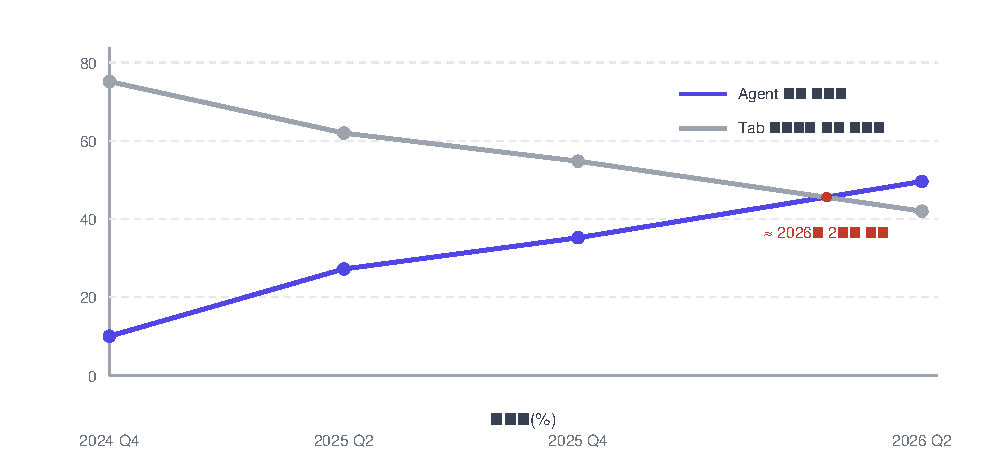
\includegraphics[width=0.92\linewidth]{figures/fig-di-san-shi-qi-zhang-1}
\\[2pt]\small 그림 1: AI 프로그래밍 상호작용 모드 사용률 변화 추이(업계 조사 데이터 기반 추정, 2026년 2분기에 Agent 모드가 Tab 자동완성을 추월)
\end{center}

그런데 솔직히 말하자면, 도구와 모델의 변화는 겉모습에 불과해요. Cursor를 쓰든 Claude Code를 쓰든, 기반 모델이 GPT-5든 Claude 4.5든, 성공적인 AI 프로그래밍 실천가들은 모두 같은 저변의 방법론을 따르고 있어요. 바로 이 가이드가 여러분에게 가르쳐 줄 것입니다.

\booksection{핵심 인식 전환: Coder에서 Conductor로}

전통 프로그래밍 교육은 여러분이 Coder가 되는 법, 즉 문법을 이해하고 API를 외우고 논리 오류를 디버깅하는 법을 가르쳐 줘요. AI 프로그래밍 시대에는 이 역할이 다시 정의되고 있어요. 더 이상 모든 코드를 한 줄씩 직접 작성할 필요는 없지만, '지휘관(Conductor)'이 되어야 해요. 전장을 정의하고, 규칙을 만들고, 과업을 배분하고, 성과를 검수하는 사람 말이에요.

이 전환의 핵심은 '코드를 짤 줄 아는가'가 아니라 '무엇을 할지 명확히 생각할 줄 아는가'에 있어요. 뛰어난 지휘관이 꼭 최고의 병사일 필요는 없지만, 전투의 목표와 지형, 병력 배치를 누구보다 잘 알아야 하죠. 마찬가지로 뛰어난 AI 프로그래밍 실천가가 모든 프로그래밍 언어의 문법 디테일에 정통할 필요는 없지만, 프로젝트의 목표와 아키텍처 제약, 품질 기준을 누구보다 명확히 알아야 해요.

이 표는 두 번씩 다시 볼 가치가 있어요. 이번 역할 전환의 모든 내용을 요약하고 있거든요.

\begin{center}
\begin{tabularx}{\linewidth}{|X|X|X|}
\hline
\textbf{구분} & \textbf{전통적인 Coder} & \textbf{AI 지휘관(Conductor)} \tabularnewline
\hline
핵심 역량 & 문법 암기, API 호출, 디버깅 & 요구사항 정의, 컨텍스트 관리, 검수 판단 \tabularnewline
작업 방식 & 코드를 한 줄씩 작성 & 의도를 설명하고 결과물을 검토 \tabularnewline
품질 관리 & 직접 쓴 코드라 내가 모두 파악 & 테스트와 검토로 AI 결과물을 검증 \tabularnewline
지식 요구 수준 & 특정 언어/프레임워크를 깊이 숙지 & 기술 전체를 넓게 이해하고, 비즈니스 로직을 깊이 이해 \tabularnewline
병목 지점 & 코딩 속도와 문법 암기 & 생각의 명확성과 표현력 \tabularnewline
오류의 원인 & 문법 오류, 논리 누락 & 요구사항이 모호함, 컨텍스트 부족 \tabularnewline
\hline
\end{tabularx}
\end{center}

\begin{center}\small\color{gray}전통적인 Coder와 AI 지휘관의 역량 항목 비교\end{center}

프로그래밍 지식이 이제 중요하지 않다는 뜻은 절대 아니에요. 오히려 정반대예요. AI가 쓴 코드를 읽을 줄 알아야 효과적으로 검토하고 수정할 수 있고, 자료구조와 알고리즘을 이해해야 AI의 방안이 합리적인지 판단할 수 있어요. 지식이 여러분의 '지휘 상한선'을 결정해요. 다만 지식의 역할이 '실행 도구'에서 '판단 근거'로 바뀐 거죠.

\booksection{왜 방법론이 도구보다 더 중요할까요?}

도구는 세 달마다 바뀌지만, 방법론은 세 년에 한 번 진화해요. 도구 조작을 익히면 세 달 뒤엔 낡았을 수 있지만, 사고방식 한 세트를 익히면 세 년 뒤에도 여전히 통해요.

많은 사람이 AI 프로그래밍에 입문할 때 가장 먼저 '어떤 도구가 제일 좋아요?', '어떤 모델이 제일 강해요?'를 묻곤 해요. 그런 질문이 중요하지 않다는 게 아니라, 우선순위를 잘못 묻고 있는 거예요. 2026년 8월의 도구 지형은 2025년 8월과 완전히 달라졌어요. Trae, Qoder 같은 도구들이 흥하고 망하고를 반복했고, Cursor는 플러그인에서 독립 IDE로, 다시 Cursor 3로 진화했으며, Claude Code는 실험적 프로젝트에서 터미널 프로그래밍의 주류 선택이 되었죠. 하지만 이 격변 뒤에서 성공적인 실천가들이 지키는 사고 원칙은 거의 변하지 않았어요.

그래서 이 책은 특정 도구의 조작법을 가르치는 데 지면을 쓰지 않아요. 그런 내용은 쓰는 순간 곧 낡아 버리니까요. 대신 이 책의 모든 무게는 검증된 사고 방법론에 실려 있어요. 요구사항을 어떻게 생각할지, AI와 어떻게 소통할지, 결과물을 어떻게 검증할지, 어떻게 계속 반복 개선할지 말이에요. 이 방법론만 익히면 어떤 도구로 바꿔도 빨리 적응할 수 있고, 도구 조작만 배웠다면 도구를 바꿀 때마다 처음부터 다시 배워야 해요.

\begin{tcbinfo}{기초가 없는 독자를 위한 안심 메시지}
기초가 전혀 없어도 '방법론'이라는 세 글자에 겁먹지 마세요. 방법론은 추상적인 철학이 아니라 '문제를 만났을 때 어떻게 생각할지'에 대한 실전 매뉴얼이에요. 요리 배움에 비유하면, 레시피를 따라 한 단계씩 할 수도 있지만(도구 조작) 진짜 셰프는 '왜 이렇게 간을 하는지', '불 조절을 어떻게 하는지'(방법론)를 이해하고 있죠. 이 책은 가장 기초적인 개념부터 설명하고, 모든 원칙에 구체적인 비교 사례를 곁들여서 '무엇인지'뿐 아니라 '어떻게 하는지'까지 확실히 익히도록 도울 거예요.

\end{tcbinfo}

\begin{tcbpractice}{직접 해 보기: 지금의 나에게 '역할 사진' 찍어 주기}
종이 한 장을 꺼내 세 가지 질문의 답을 적어 보세요. (1) 지금은 AI에게 코드를 어떻게 짜 달라고 하고 있나요(써 본 적 있다면)? (2) 위 표에서 나는 'Coder'에 가까운가요, '지휘관'에 가까운가요? (3) 세 달 뒤의 내가 자신의 작업 방식을 어떻게 묘사했으면 좋겠나요? 다 쓰면 책에 끼워 두고, 제47장을 다 읽고 나서 다시 꺼내 보세요. 생각보다 빨리 변했다는 걸 알게 될 거예요.

\end{tcbpractice}

\begin{tcbsummary}{이번 장 정리}
\begin{itemize}
  \item 2025년 Karpathy가 'Vibe Coding'이라는 이름으로 AI 프로그래밍 혁명을 명명했어요: 한 줄씩 코드를 쓰는 방식에서 자연어로 의도를 설명하는 방식으로
  \item 2026년에는 Agentic Engineering으로 진화했어요: 목표를 주고 권한을 넘기면 AI가 스스로 계획·실행하고, 사람은 검수를 담당
  \item Cursor 3의 Agent 모드 사용률이 처음으로 Tab 자동완성을 추월했고, Claude Code는 연환산 수익 25억 달러를 달성했어요
  \item 여러분의 새 역할은 Conductor(지휘관)예요: 전장을 정의하고, 규칙을 만들고, 과제를 배분하고, 성과를 검수해요
  \item 도구는 3개월마다 바뀌고, 방법론은 3년에 한 번 진화해요. 조작법이 아니라 방법론을 배우세요
\end{itemize}

\end{tcbsummary}
